\begin{align}
    \label{eq:Cw1}
    C_w=\frac{\frac{m_{PFCA}-m_{w}}{m_{BC}}}{\frac{m_{BC}\cdot K_d}{V_w}+1}
\end{align}

Where:\newline
\begin{tabular}{p{1.5cm}p{20cm}}
$C_w$ & is the PFCA concentration in the water phase (\textmu g/L),\\
    $C_s$ & is the PFCA concentration in the solid (biochar) phase (\textmu g/g)\\
    $K_d$ & is the char-water partition coefficient (L/g), \\
\end{tabular}

\subsubsection{Biochar}
Homogeneity of the biochar samples could be a relevant source of error. The biochar was only crushed and not sieved. The biochar was only sieved to check for particle size range after the sorption experiments were set up. Most of the particles were \textless1 mm, however, some were larger, so the biochar samples may have some variation in particle size for each batch test.

%rewrite because all are below 1 mm%

\begin{table}
    \centering
    \caption{Concentration range over four orders of magnitude used for each PFCA compound in the batch sorption experiments. These concentrations are the initial water concentration prior to sorption by biochar. }
    \label{tab:concentration_range}
    \begin{tabular}{lrcr} \toprule
    Compound & \multicolumn{3}{c}{\begin{tabular}[c]{@{}c@{}}Concentration\\ range (\textmu l/L)\end{tabular}} \\ \midrule
    PFPeA & 0.030 & - & 300 \\
    PFHxA & 0.060 & - & 600 \\
    PFHpA & 0.013 & - & 130 \\
    PFOA & 0.120 & - & 1200 \\
    PFNA & 0.160 & - & 1600 \\
    PFDA & 0.500 & - & 5000 \\ \bottomrule
    \end{tabular}
\end{table}


\begin{table}
    \caption{Spike concentrations for each PFCA batch test.}
    \label{tab:concentrations}
    \adjustbox{max width=\textwidth}{%
    \begin{tabular}{llllllllllllll}
    \toprule
    & \multicolumn{13}{c}{{[}PFAS{]}   (\textmu g/L) in standards} \\ \midrule
    Compound & C1 & C2 & C3 & C4 & C5 & C6 & C7 & C8 & C9 & C10 & C11 & C12 & C13 \\ \midrule
    PFPeA & 0.03 & 33 & 68 & 100 & 135 & 168 & 200 & 235 & 268 & 300 & 5 168 & 103 & 15 \\
    PFHxA & 0.06 & 68 & 133 & 200 & 265 & 335 & 400 & 465 & 530 & 600 & 14 201 & 284 & 21 \\
    PFHpA & 0.01 & 13 & 28 & 43 & 57 & 73 & 88 & 103 & 118 & 130 & 3 360 & 27 & 10 \\
    PFOA & 0.12 & 132 & 267 & 400 & 535 & 668 & 800 & 935 & 1 070 & 1 200 & 13 920 & 557 & 13 \\
    PFNA & 0.16 & 178 & 355 & 535 & 711 & 890 & 1 070 & 1 245 & 1 425 & 1 600 & 18 360 & 367 & 10 \\
    PFDA & 0.50 & 555 & 1 110 & 1 665 & 2 220 & 2 775 & 3 330 & 3 885 & 4 440 & 5 000 & 17 100 & 684 & 10 \\ \bottomrule
    \end{tabular}}
\end{table}

\begin{figure}
     \centering
     \begin{subfigure}[t]{\linewidth}
         \centering
         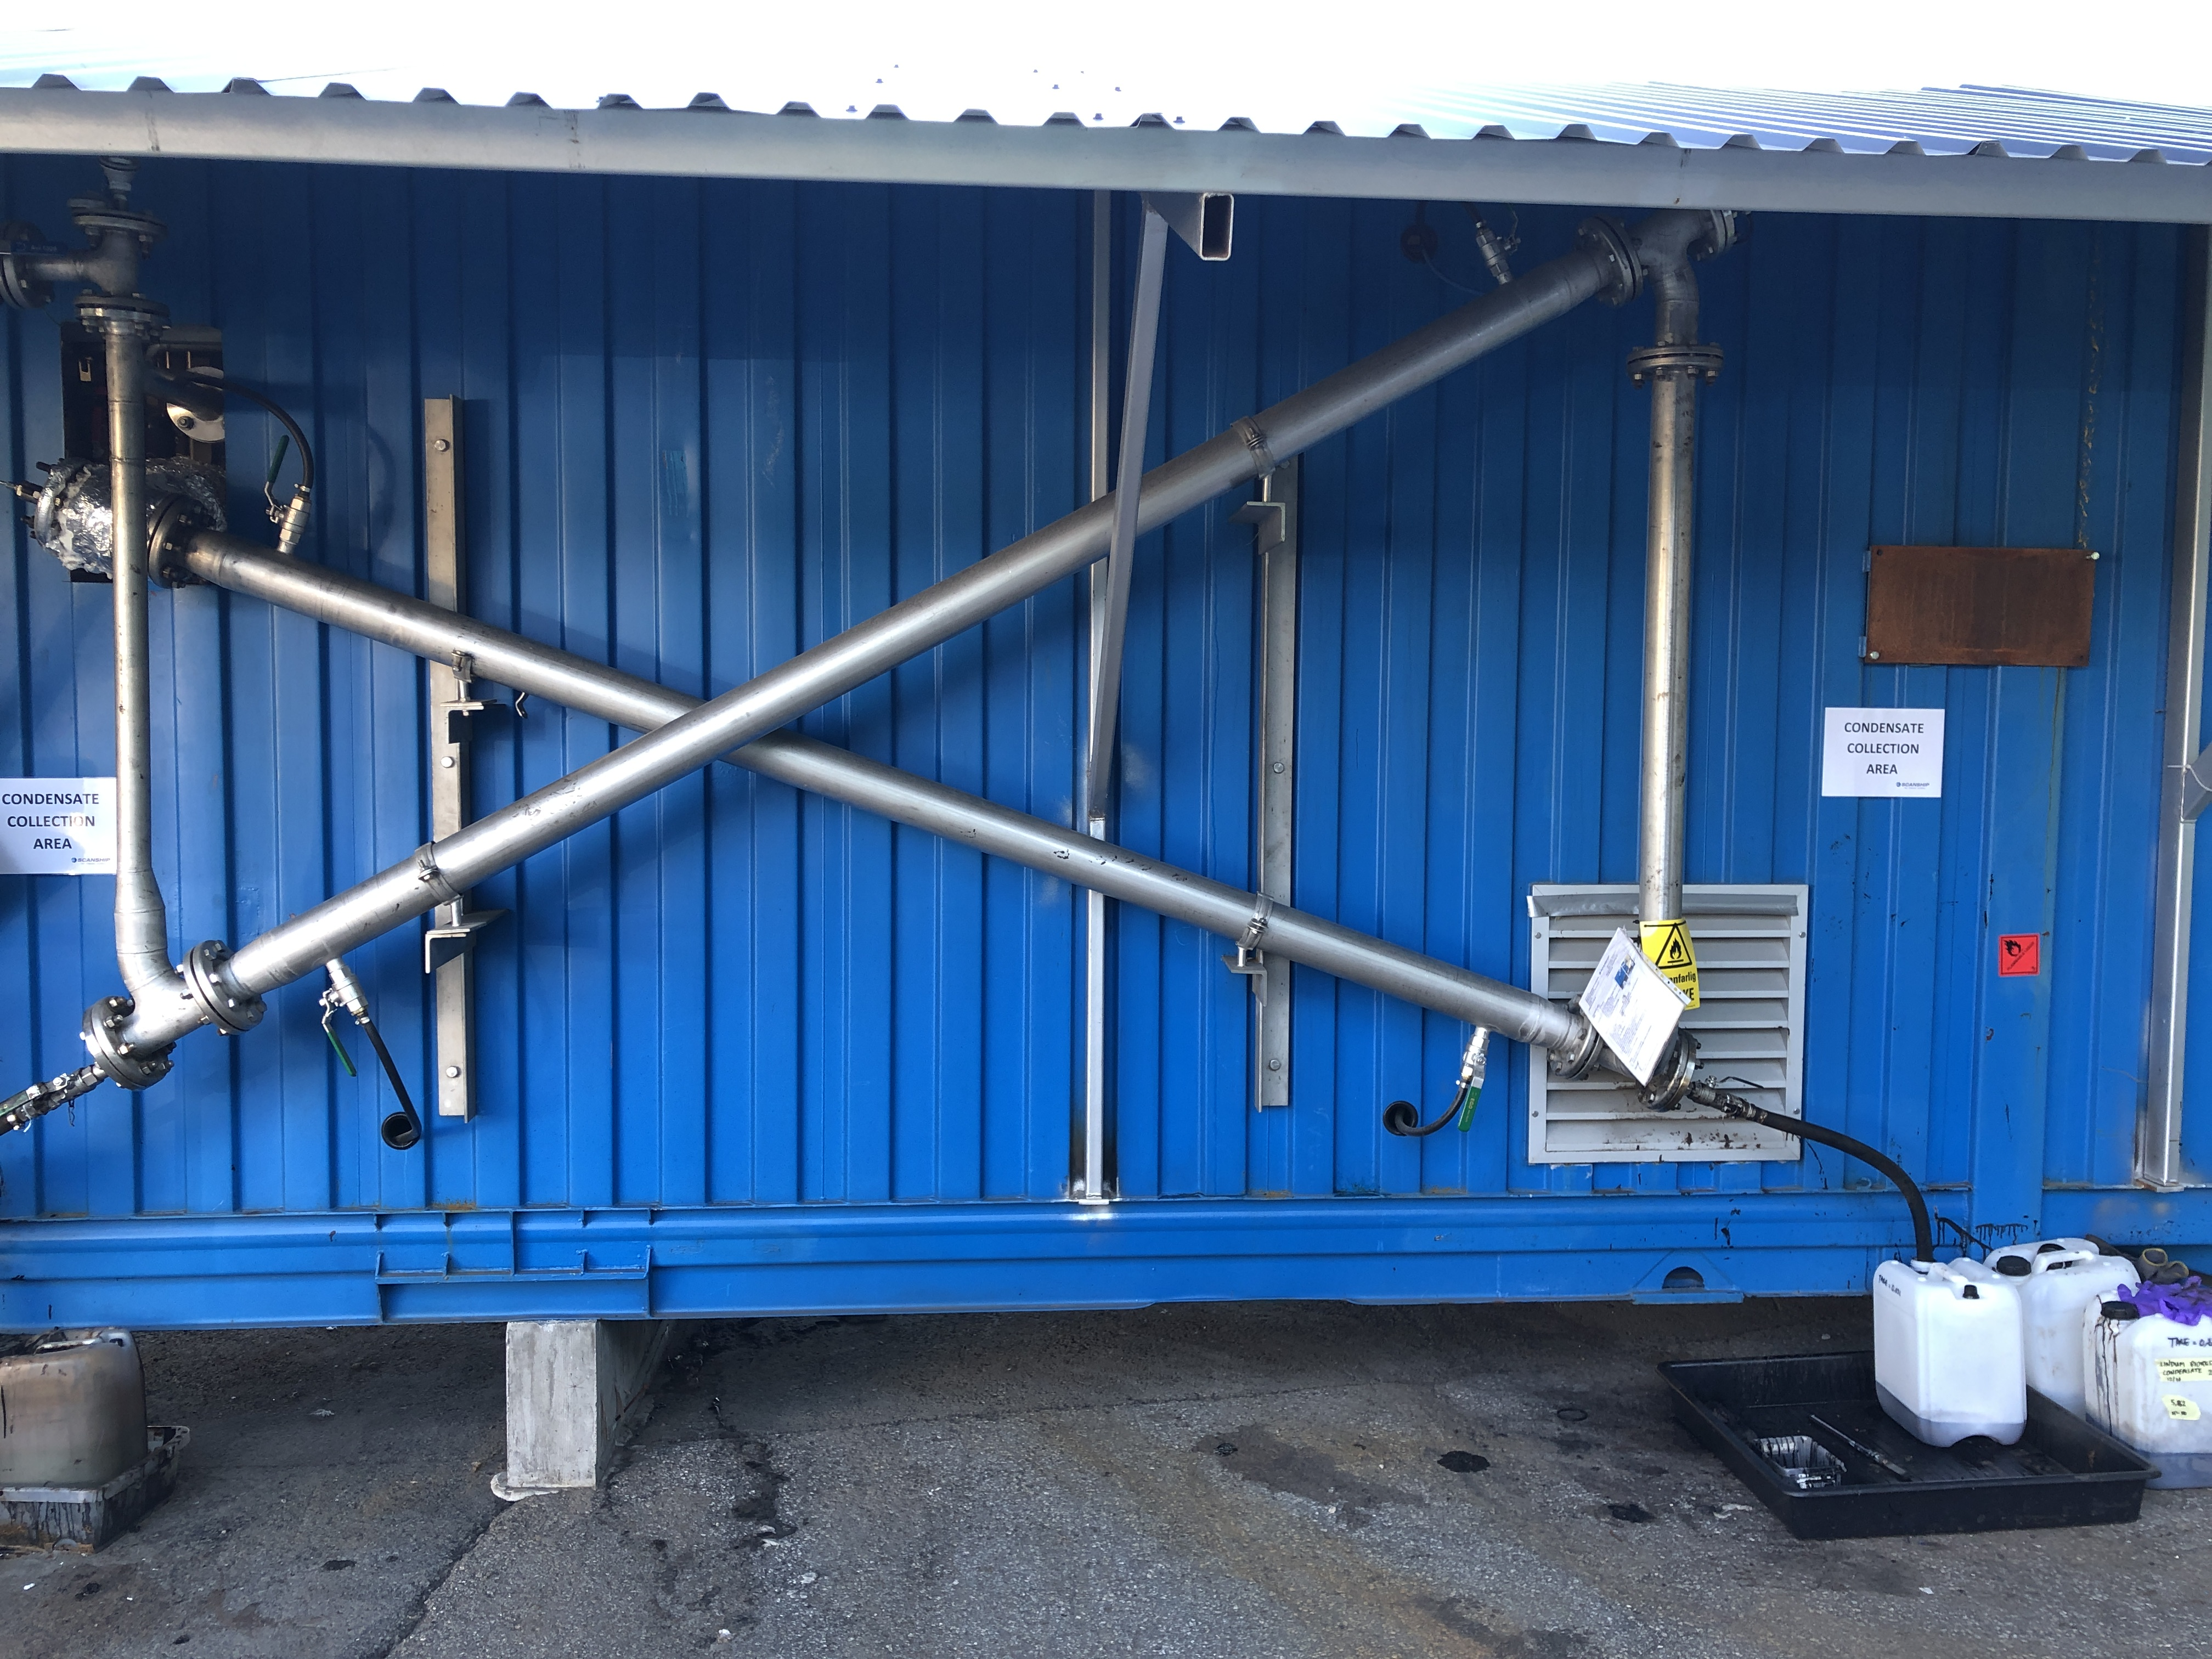
\includegraphics[width=0.6\linewidth,scale=0.6]{Bilder/Pyrolysis/Condenser.png}
         \hspace{0.5 cm}
         \caption{}
         \label{fig:condenserfull}
     \end{subfigure}
     \hfill
     \begin{subfigure}[b]{0.3\linewidth}
         \centering
         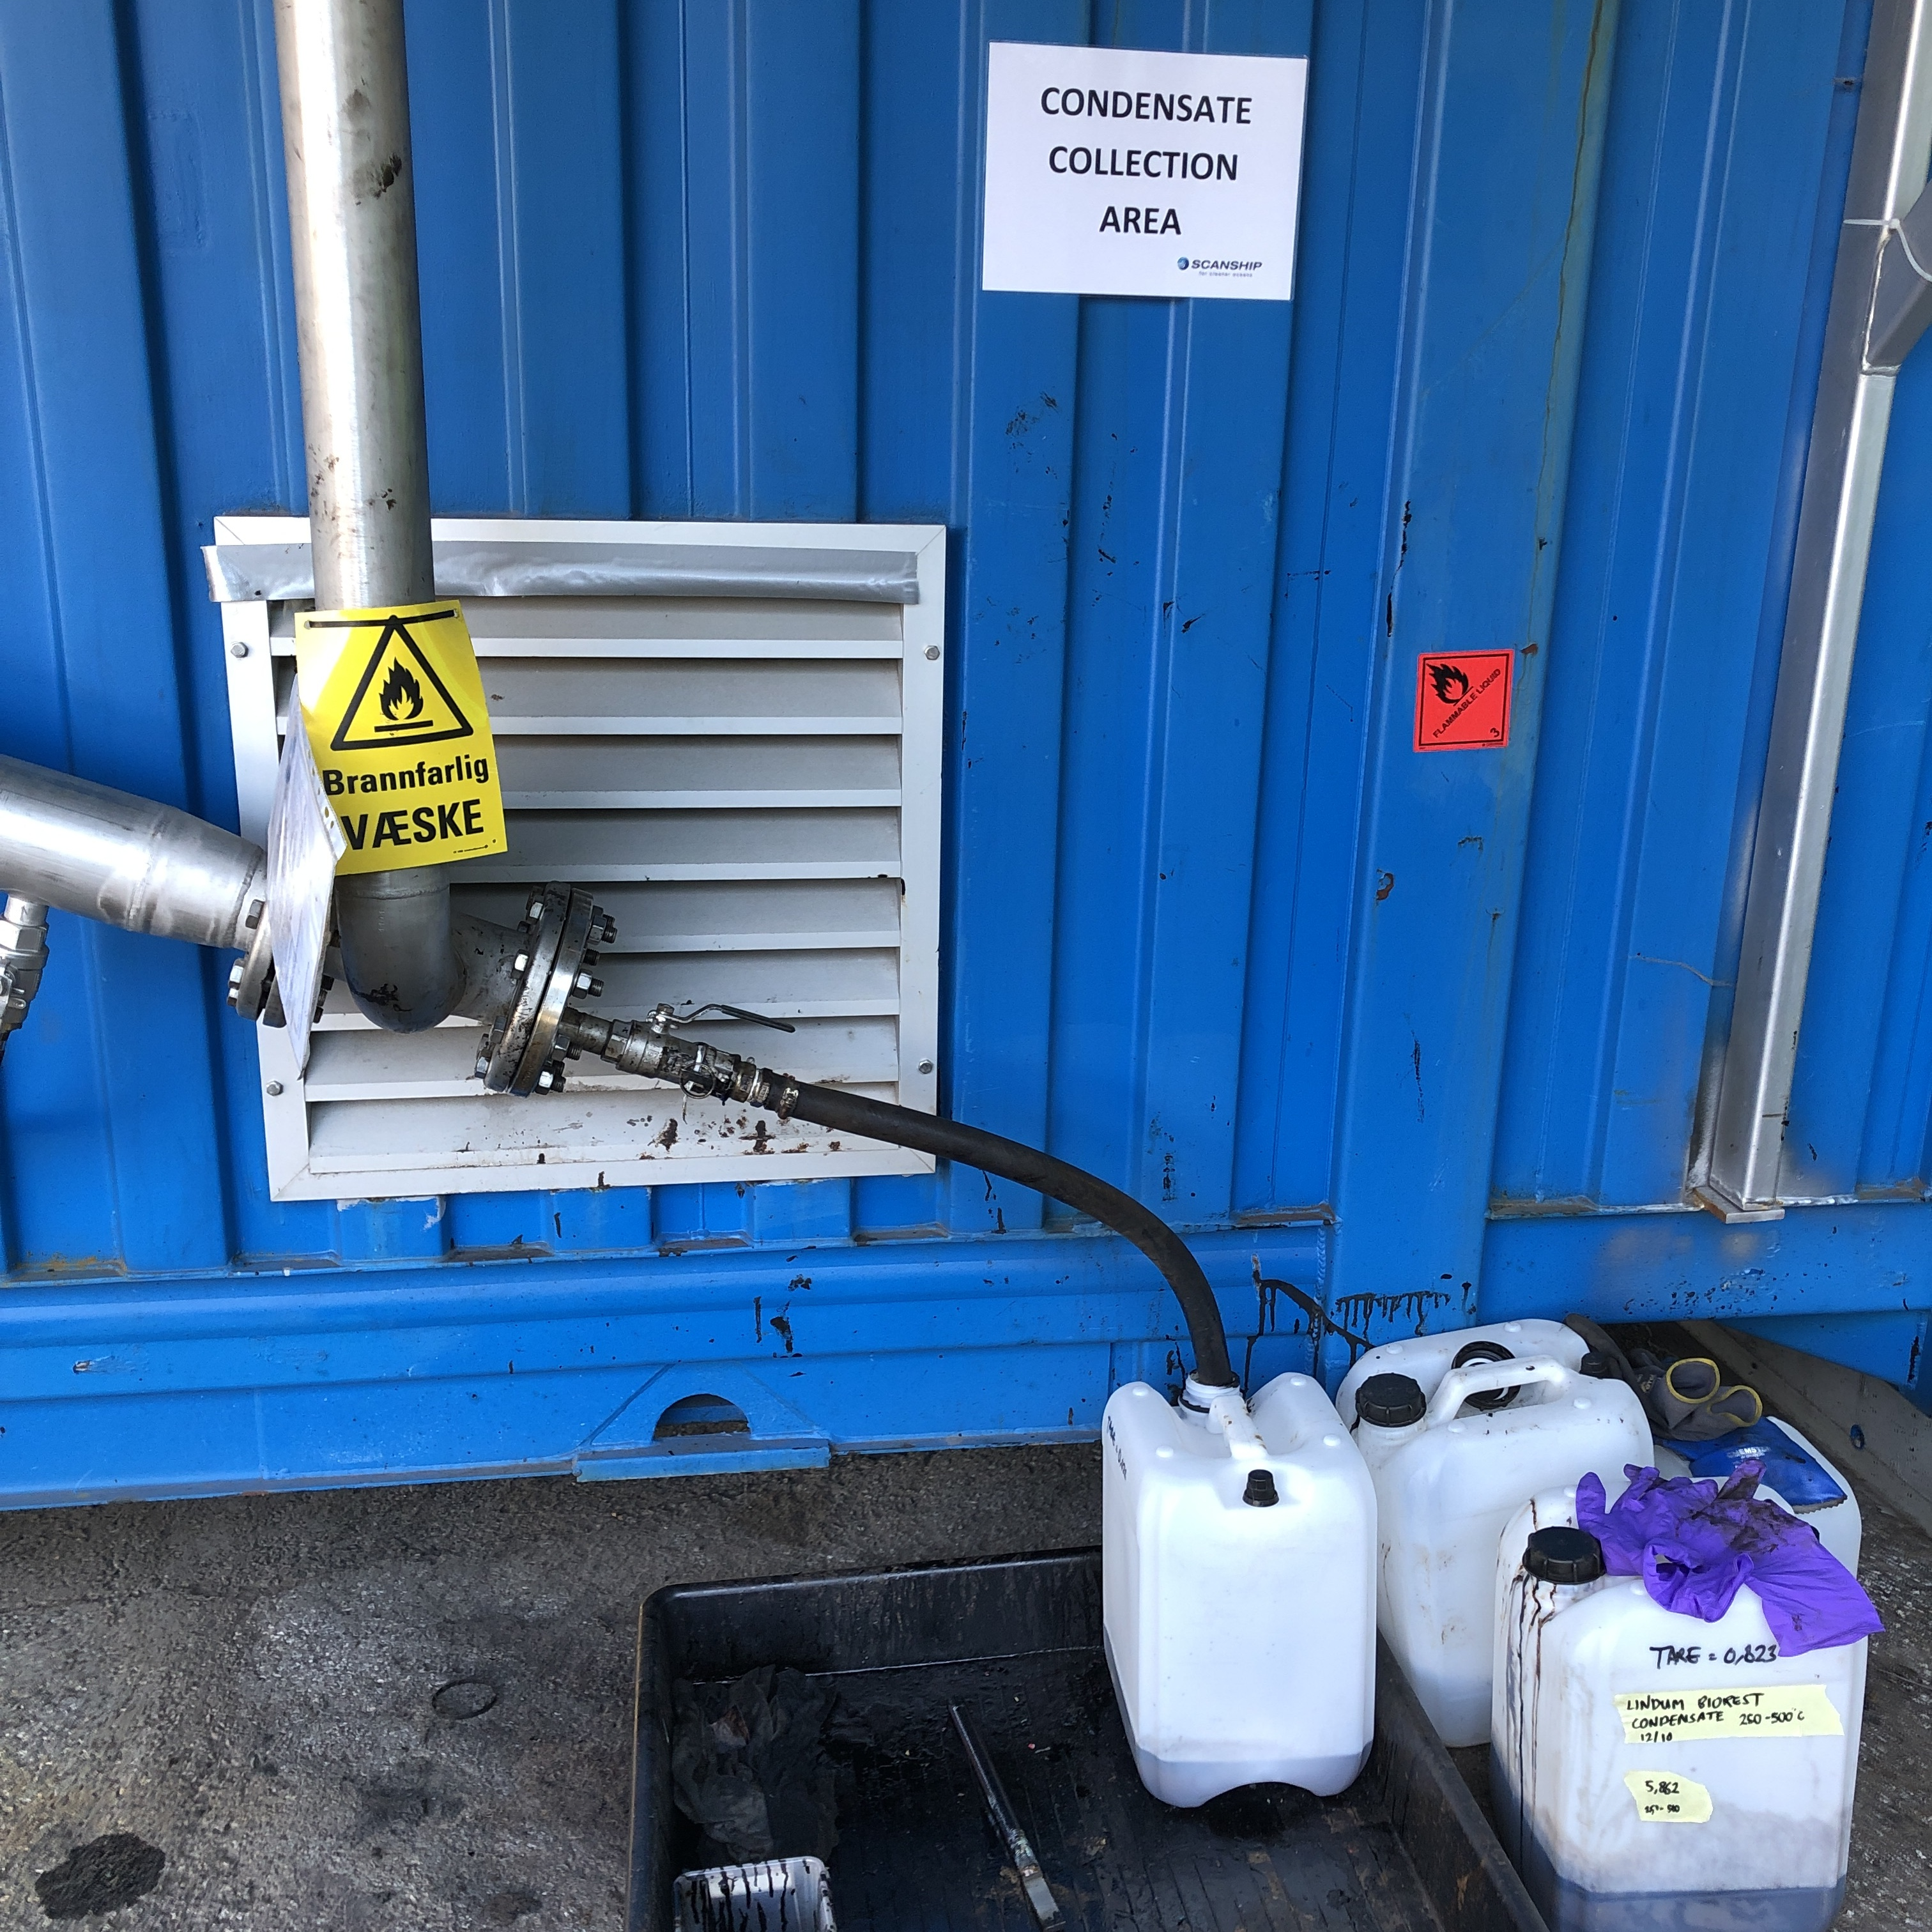
\includegraphics[width=\linewidth]{Bilder/Pyrolysis/CondensateCollection1.jpg}
         \caption{}
         \label{fig:condensate1}
     \end{subfigure}
     \hfill
     \begin{subfigure}[b]{0.3\linewidth}
         \centering
         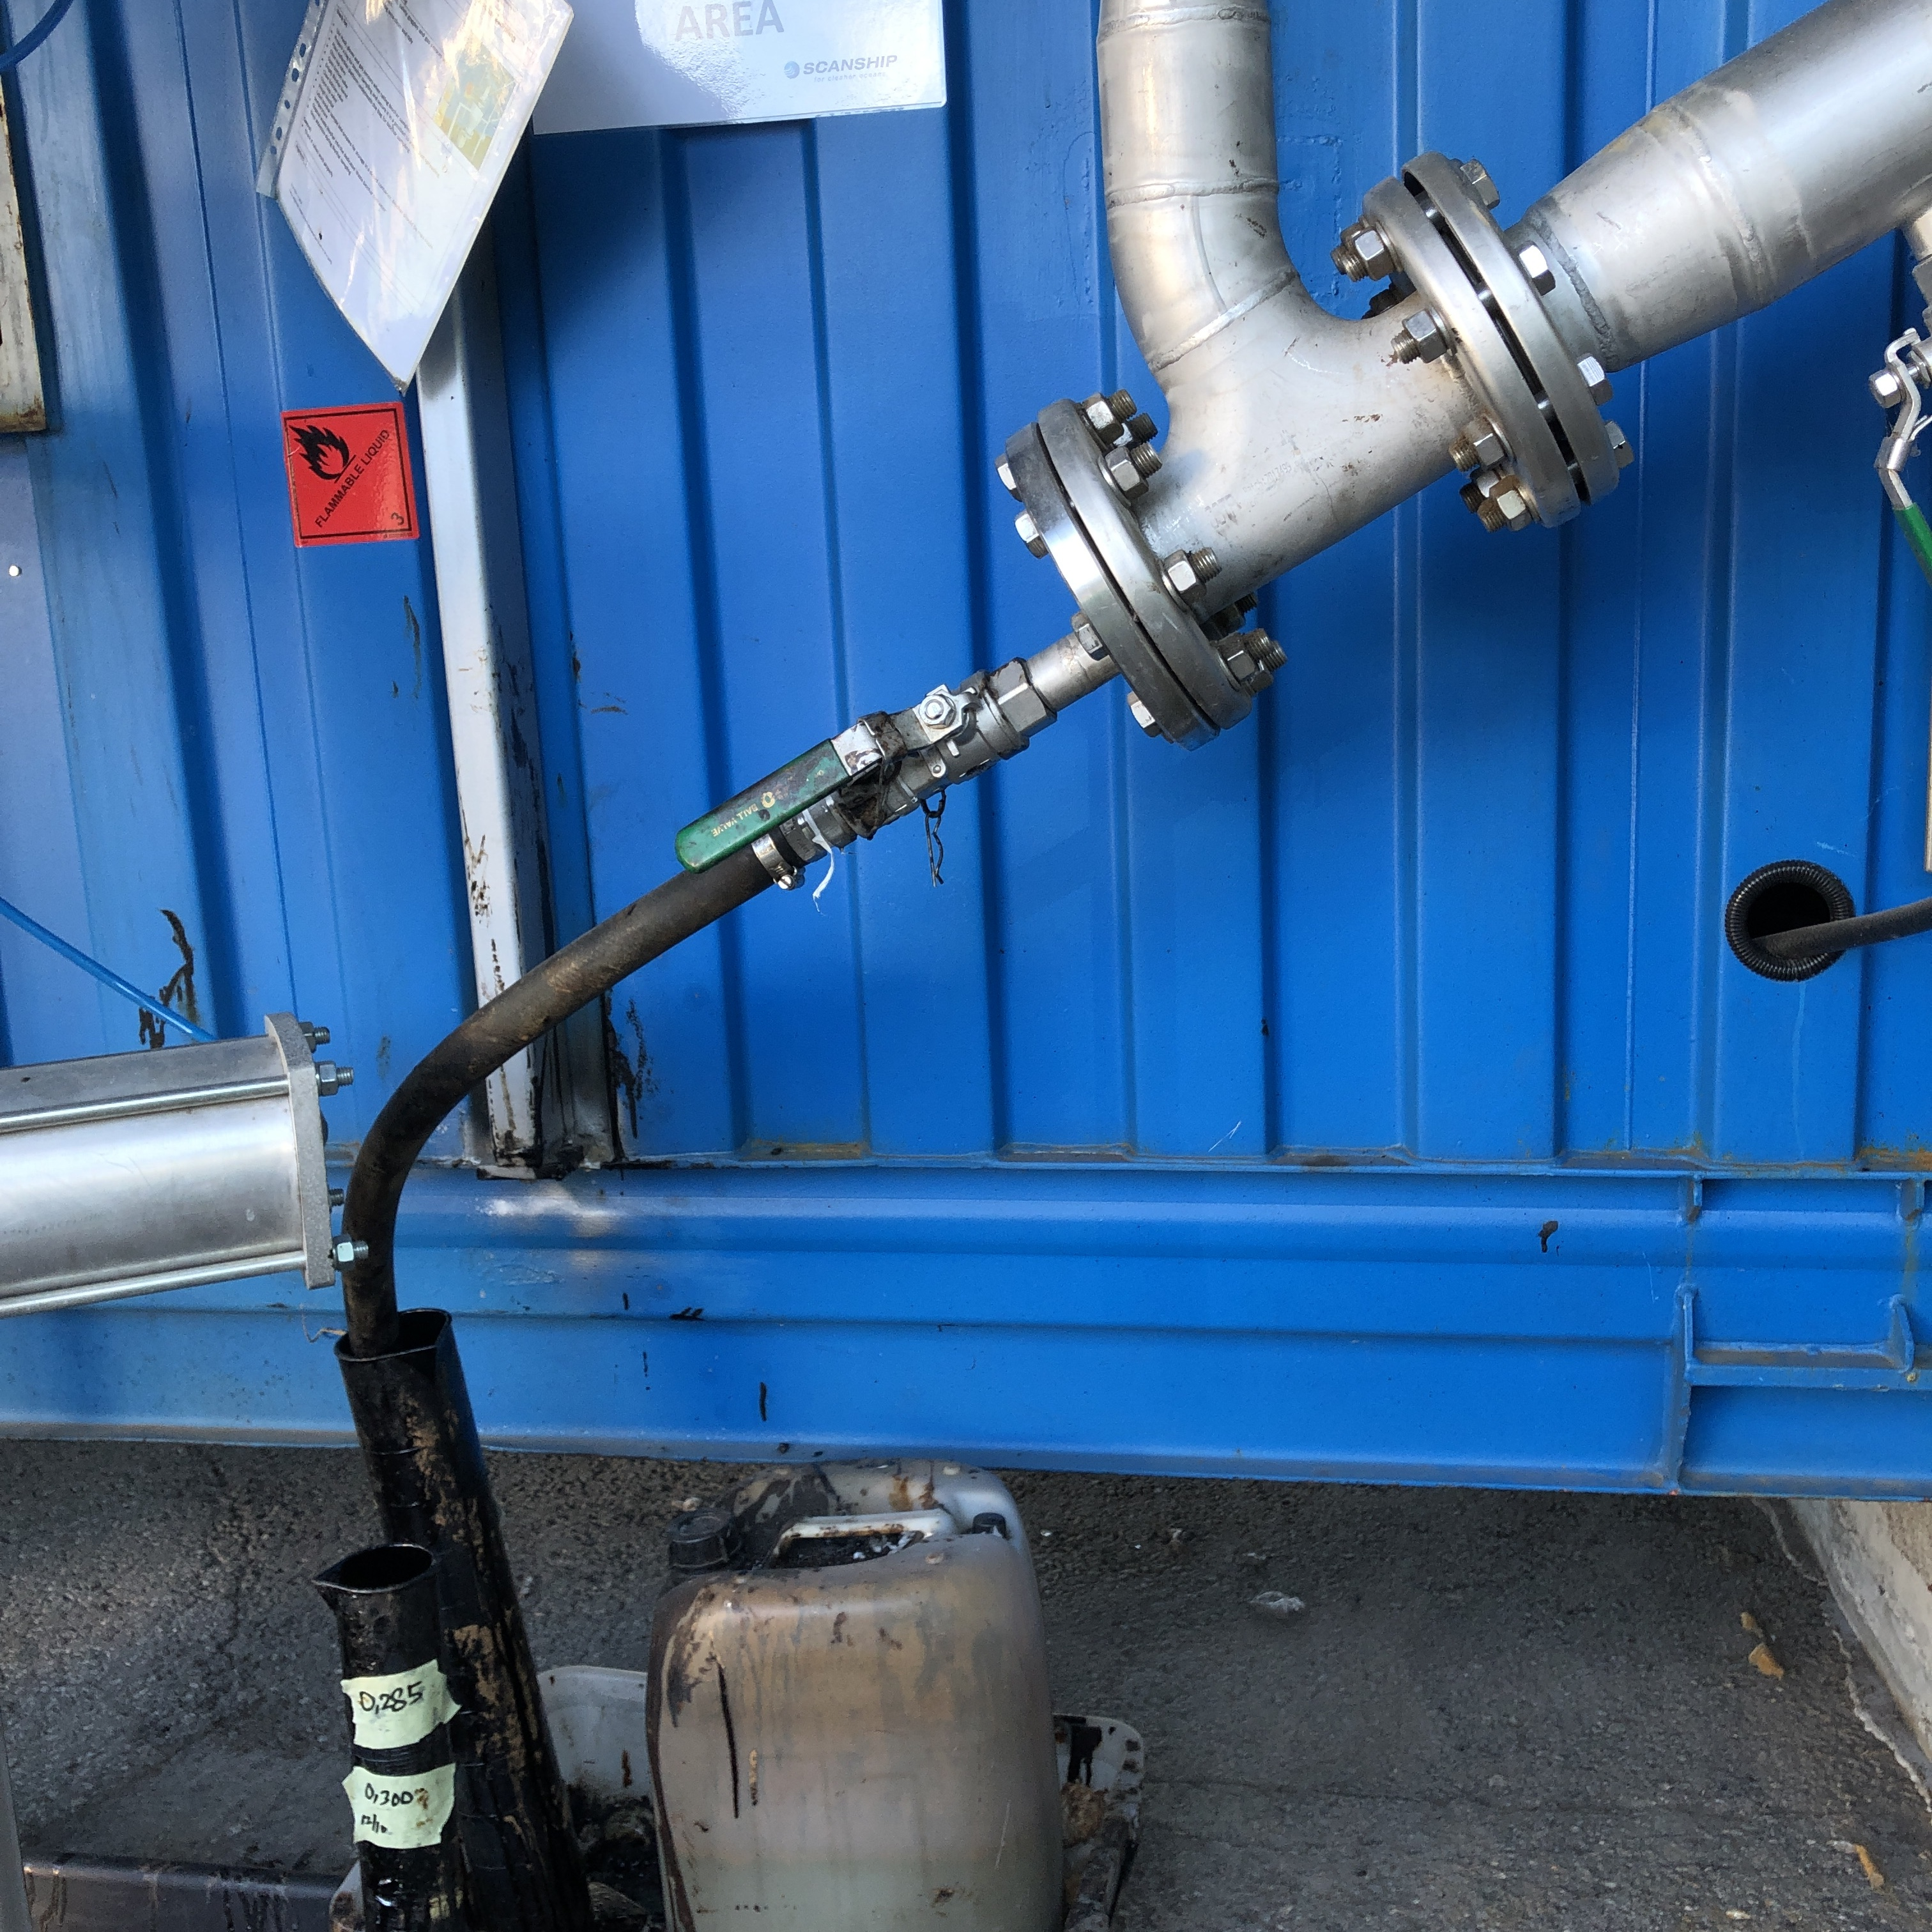
\includegraphics[width=\linewidth]{Bilder/Pyrolysis/CondensateCollection2.jpg}
         \caption{}
         \label{fig:condensate2}
     \end{subfigure}
        \caption{Syn-gas condenser. (a) First condensate collection area draining long-chain bio-oils. (b) Second condensate collection area draining short-chain bio-oils.}
        \label{fig:condenser}
\end{figure}

\begin{table}
    \centering
    \caption{Purity, stock form and LOQs of the PFCAs used for the sorption isotherms. iLOQ = instrumental LOQ for  the extract, mLOQ = method LOQ.}
    \label{tab:PFCAform&LOQ}
    \begin{tabular}{@{}lllccc@{}}
    \toprule
    \multicolumn{1}{l}{Compound}  & \multicolumn{1}{l}{Purity}  & \multicolumn{1}{l}{Stock form} & \multicolumn{1}{l}{iLOQ} & \multicolumn{1}{l}{mLOQ}  & \multicolumn{1}{l}{2$\times$mLOQ}\\ 
    & & & \multicolumn{1}{l}{(ng mL\textsuperscript{-1})}  & \multicolumn{1}{l}{(ng L\textsuperscript{-1})}  & \multicolumn{1}{l}{(ng L\textsuperscript{-1})} \\ \midrule
     PFPeA  & 97 \%   & liquid    & 0.05 & 0.50  & 1.00     \\
     PFHxA  & 97 \%   & liquid    & 0.10 & 1.00   & 2.00     \\
     PFHpA-K  & 99 \%   & crystalline & 0.01 & 0.10   & 0.20    \\
     PFOA-K   & 95 \%   & powder    & 0.05 & 0.50    & 1.00   \\
     PFNA-K   & 97 \%    & crystalline  & 0.05 & 0.50 & 1.00   \\
     PFDA-K   & 98 \% & flakes & 0.10 & 1.00 & 2.00  \\ \bottomrule
    \end{tabular}
\end{table}

 The cartridges used for extraction of PFAS  Strata\textsuperscript{\textregistered}-X Phenomenex: Cartridges with  200 mg/6mL 
 
 Gabi
 Determination of target analytes was performed in an UPLC-MS/MS with a Xevo TQ-S triple quadrupole mass spectrometer furnished with a ESI Z spray, and connected to an Acquity UPLC I-Class system, both acquired from Waters (Milford, MA, U.S.). Chromatographic separation was carried out in a Kinetex C18 column (30 x 2.1 mm, 1.3 μm) serially connected to a C18 (2 x 2.1 mm i.d.) security guard, both supplied by Phenomenex (Torrance, CA, U.S.). Milli-Q water 2 mM ammonium acetate (A) and pure MeOH (B), were used as mobile phases at a constant flow rate of 250 μL min-1. The UPLC column and precolumn were maintained at 30 ºC. The mobile phase gradient was programmed as follows: 0-0.2 min, 10\% B; 3.0-3.5 min, 100\% B; 3.6-5 min, 10\% B. The injection volume was 4 μL. Analytes were ionized under negative ionization mode (ESI-). Nitrogen was used as drying gas at the ionization source (450ºC at 650 L hour-1). The capillary voltage was maintained at 2 kV, the cone voltage at 25 V, and the source offset voltage at 40 V. Two transitions were monitored per chemical (Table 1) considering a time window of 60 s around their retention time. The dwell time per transition was automatically adjusted by the MassLynx software to obtain 12 points per peak assuming an average baseline peak width of 5 s. 
UPLC-MS/MS data was acquired with MassLynx version 4.1 software, while quantification processing was performed with TargetLynx (Waters, Milford, U.S.).

Procedural blank: IS spiked directly into cartridge and eluted with methanol to check contamination during the extraction protocol. If the reagent blank is contaminated, the signal must be subtracted from the rest of the samples. 
Three matrix matched samples with the same concentrations as the pre-extraction spikes that were submitted to the entire protocol where the addition of IS and analytes were made post-extraction, just to calculate recoveries \cref{eq:Recovery,eq:ME}.
Gabi:
%Contamination arising from sampling and laboratory materials was evaluated through the analysis of sampling and procedural blanks. Working benches were cleaned with acetone and covered with aluminum foil before sample preparation. In addition, clean PP material was used during the complete protocol. During analysis, solvent blanks, and a mixture of standards of 10 ng mL-1 were injected every 15 injections along the sequence to check for any potential cross contamination or sample carryover, and to evaluate signal variations and potential drifting time. A solution of MeOH:Milli-Q (50:50; v/v) 0.1 \% formic acid was used as wash solution for cleaning the injection needle during 8 and 10 seconds before and after each injection.

%A 10-point calibration curve with concentrations ranging from 0.01 to 20.0 ng mL-1 (0.01, 0.05, 0.10, 0.20, 0.50, 1.00, 2.00, 5.00, 10.0, and 20.0 ng mL-1) was prepared, and demonstrated a satisfactory regression coefficient for every target analyte (R2 > 0.98). Pre- and post- extraction spiked matrix samples were used as QA/QC samples and were prepared by spiking known amounts of the target analytes and internal standards prior and post to the sample preparation, respectively. The extraction recoveries of the method were assessed in pooled matrix at three different amounts (2.5, 5, 10 ng mL-1; n=3 replicates per amount). Matrix effects (MEs, \%) during measurements were assessed and estimated as XXXX. Quantification of the target analytes was accomplished based on the internal standard method and with matrix-matched calibration standards.

%Contamination arising from sampling and laboratory materials was evaluated through the analysis of sampling and procedural blanks. Working benches were cleaned with acetone and covered with aluminum foil before sample preparation. In addition, clean PP material was used during the complete protocol. During analysis, solvent blanks, and a mixture of standards of 10 ng mL-1 were injected every 15 injections along the sequence to check for any potential cross contamination or sample carryover, and to evaluate signal variations and potential drifting time. A solution of MeOH:Milli-Q (50:50; v/v) 0.1 \% formic acid was used as wash solution for cleaning the injection needle during 8 and 10 seconds before and after each injection.

%A 10-point calibration curve with concentrations ranging from 0.01 to 20.0 ng mL-1 (0.01, 0.05, 0.10, 0.20, 0.50, 1.00, 2.00, 5.00, 10.0, and 20.0 ng mL-1) was prepared, and demonstrated a satisfactory regression coefficient for every target analyte (R2 > 0.98). Pre- and post- extraction spiked matrix samples were used as QA/QC samples and were prepared by spiking known amounts of the target analytes and internal standards prior and post to the sample preparation, respectively. The extraction recoveries of the method were assessed in pooled matrix at three different amounts (2.5, 5, 10 ng mL-1; n=3 replicates per amount). Matrix effects (MEs, \%) during measurements were assessed and estimated as XXXX. Quantification of the target analytes was accomplished based on the internal standard method and with matrix-matched calibration standards.


\begin{figure}
    \centering
    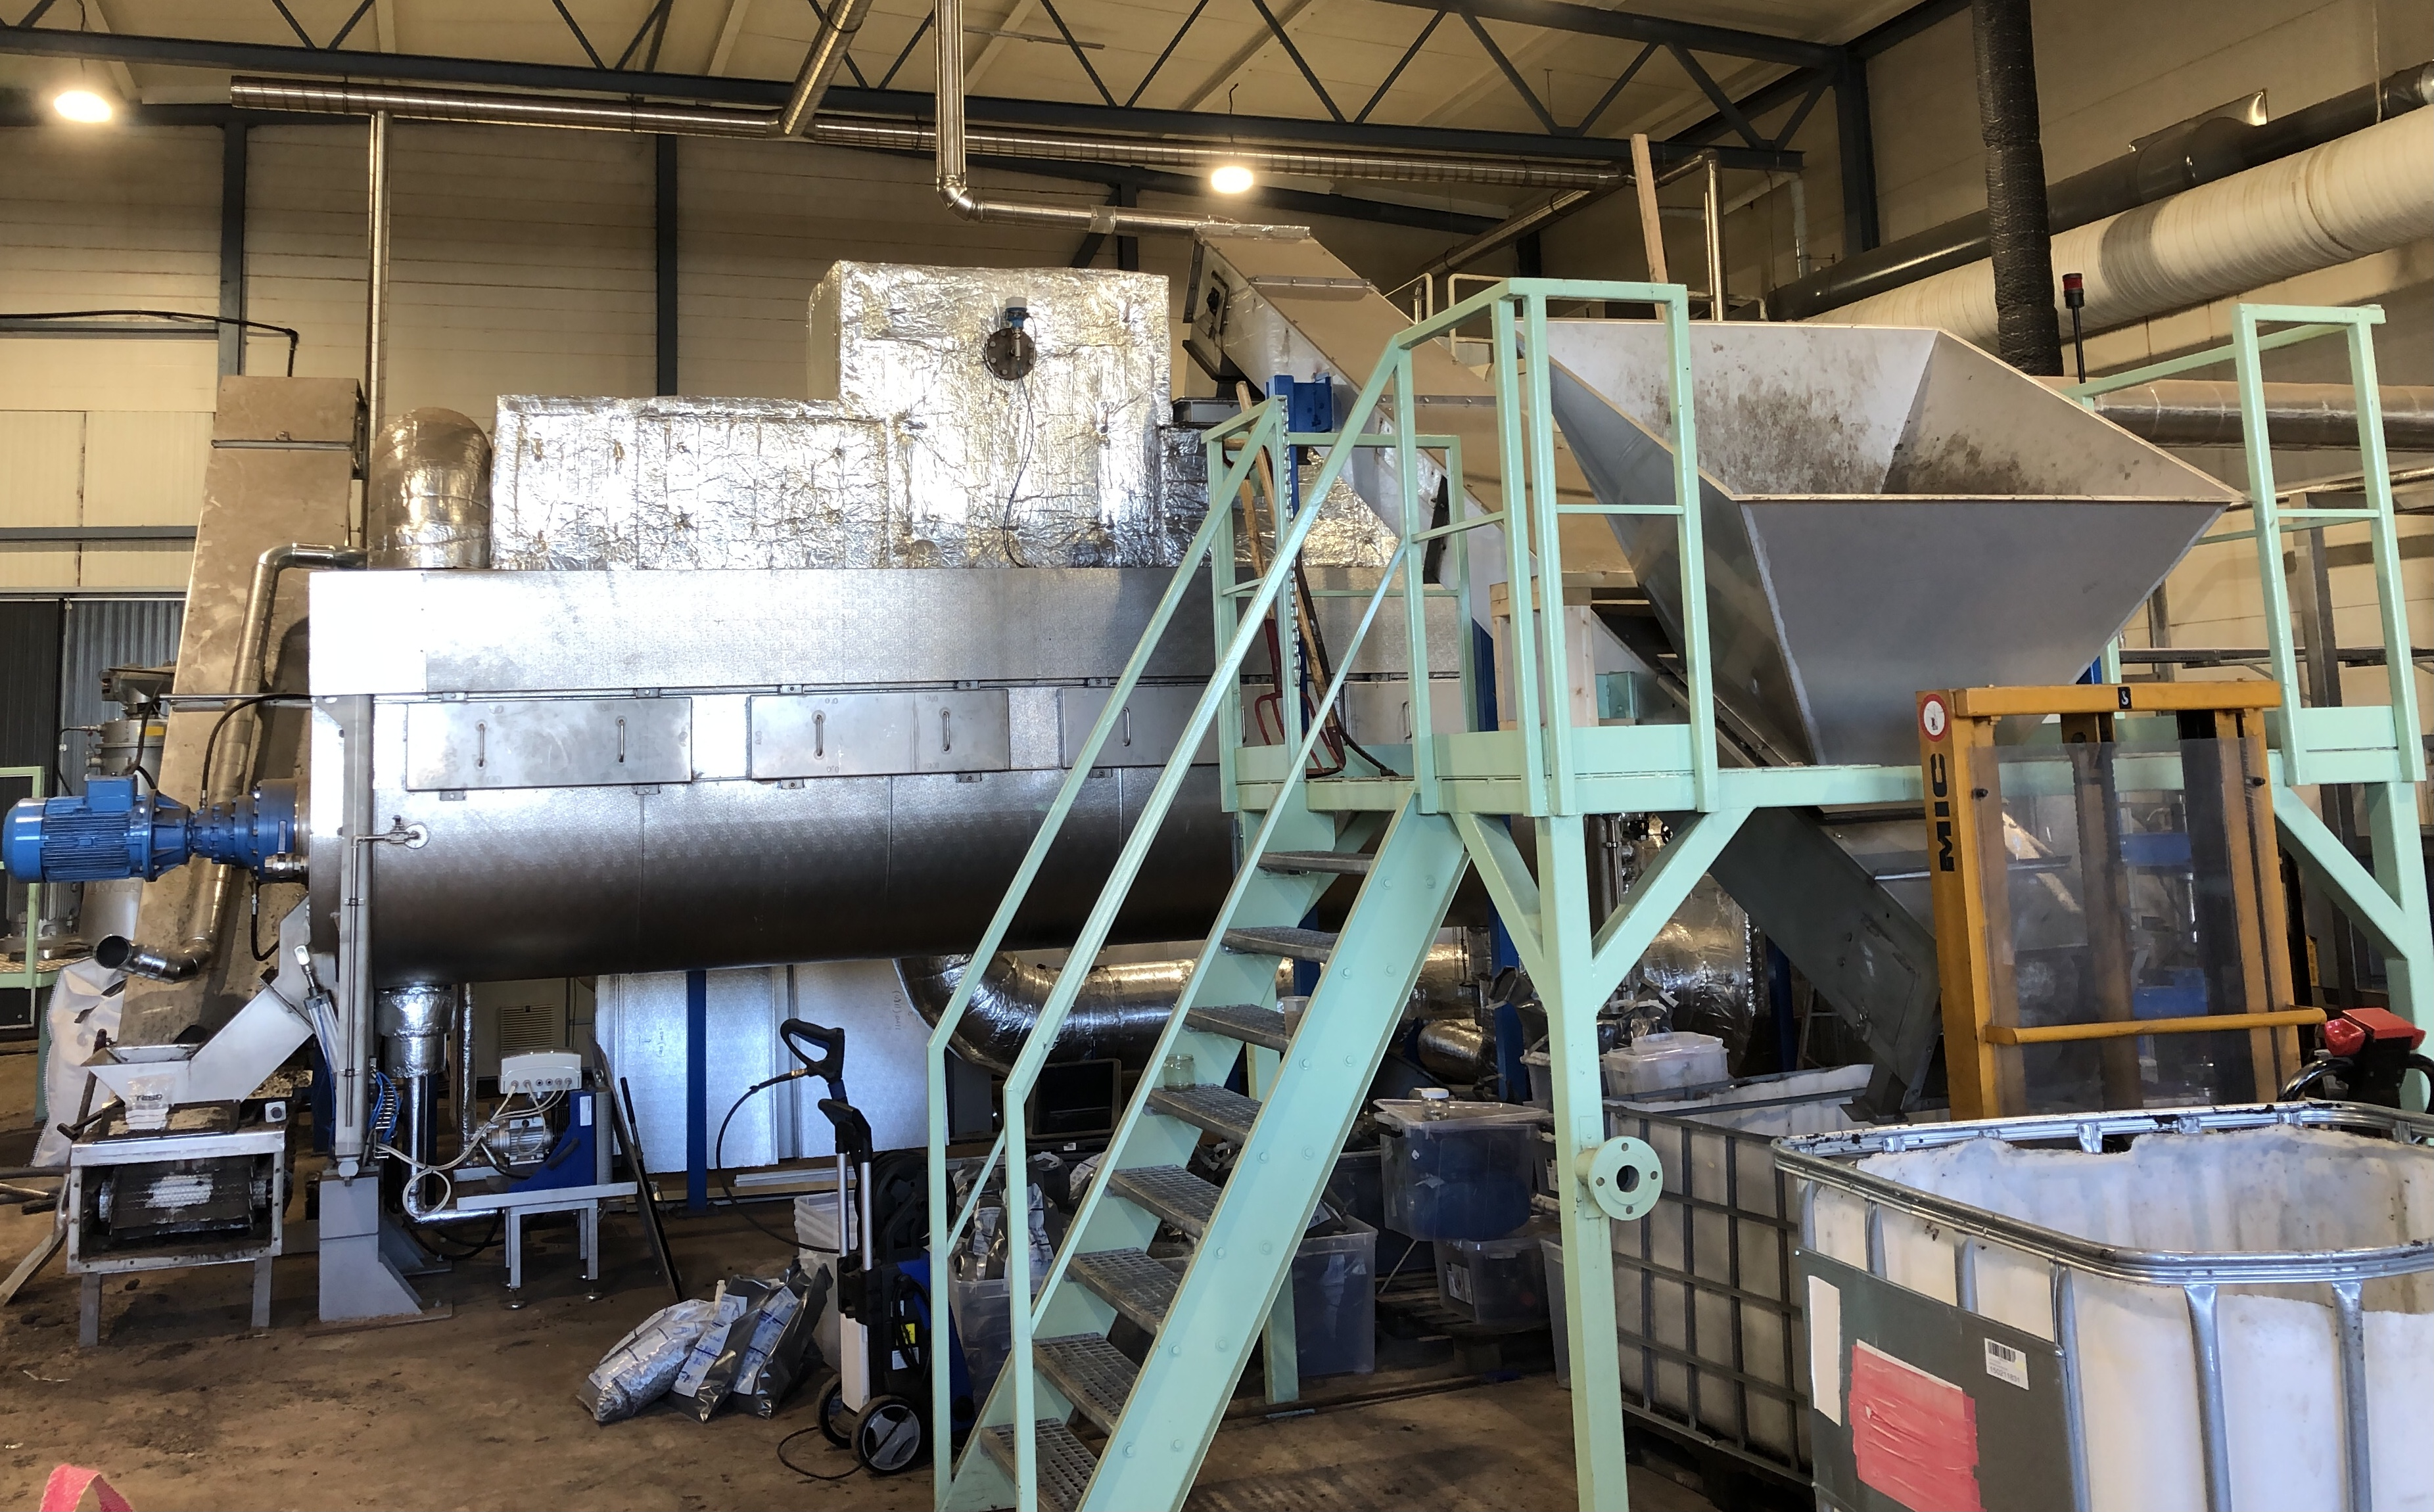
\includegraphics[width=0.7\linewidth,scale=0.7]{Bilder/Pyrolysis/Dryer.jpg}
    \caption{Sludge dryer at Lindum.}
    \label{fig:dryer}
\end{figure}

Biochar property characterization were performed at University of Florida, Gainsville\footnote{FL 32611, USA}. Iron and copper speciation was determined by XAS at the ESRF synchrotron (Grenoble, France).

\begin{figure}
    \centering
    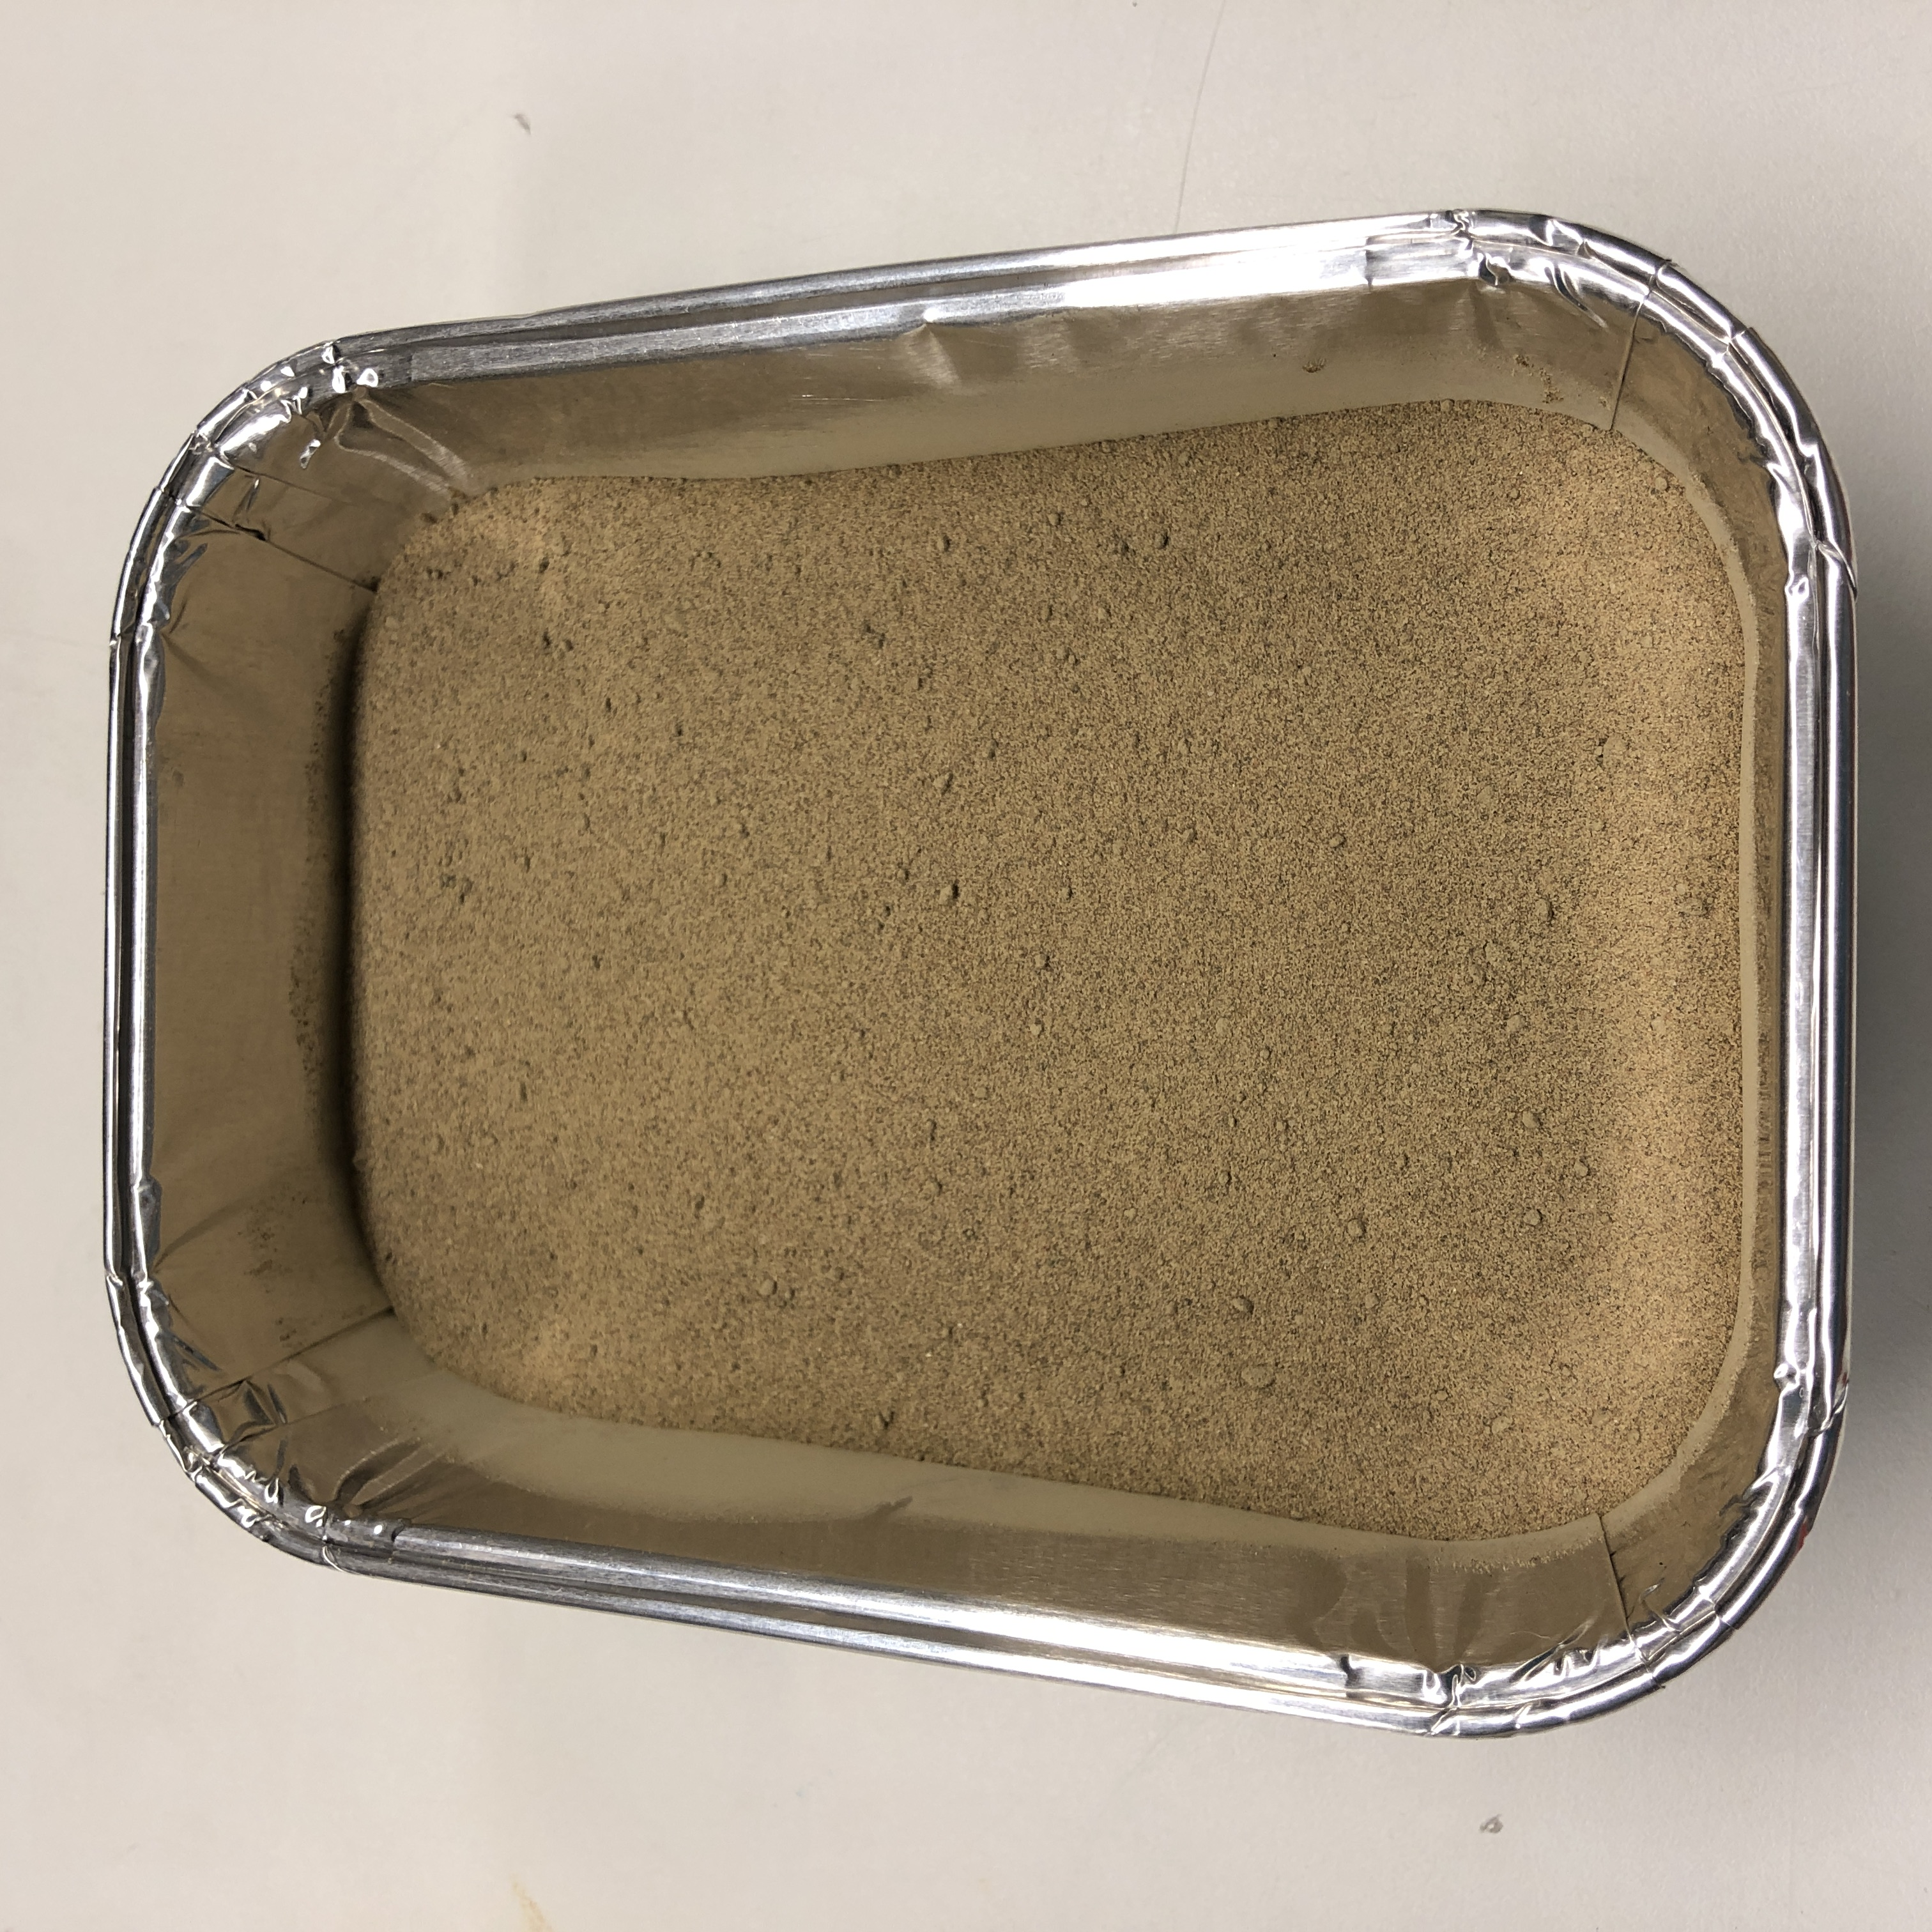
\includegraphics[width=0.5\textwidth]{Bilder/Samples/Soil_blank.JPG}
    \caption{The soil used for the batch tests.}
    \label{fig:soil}
\end{figure}